\documentclass[10pt]{article}
\usepackage[margin=0.68in]{geometry}
\usepackage{amsmath,amssymb,amsthm,mathtools}
\usepackage{tikz}
\usepackage{xcolor}
\usetikzlibrary{arrows.meta,positioning}
\usepackage{graphicx}
\usepackage{microtype}
\usepackage{enumitem}
\usepackage[hidelinks]{hyperref}
\usepackage[font=small,labelfont=bf]{caption}
% Muted Morandi-style palette for expository figures.
\definecolor{morandiTeal}{RGB}{108,139,137}
\definecolor{morandiBlue}{RGB}{104,126,155}
\definecolor{morandiSage}{RGB}{142,158,132}
\definecolor{morandiClay}{RGB}{177,132,104}
\definecolor{morandiMauve}{RGB}{155,128,146}
\definecolor{morandiLavender}{RGB}{138,132,160}
\definecolor{morandiSand}{RGB}{224,211,184}
\definecolor{morandiCream}{RGB}{246,241,231}

\setlength{\parindent}{0pt}
\setlength{\parskip}{4pt}
\setlist[itemize]{leftmargin=1.2em,itemsep=1pt,topsep=2pt}
\pagestyle{plain}

\newtheoremstyle{compactdef}{5pt}{5pt}{}{} {\bfseries}{.}{0.5em}{}
\theoremstyle{compactdef}
\newtheorem{definition}{Definition}
\newtheorem*{remark}{Remark}

\title{From Expander Codes to Higher Cubical Complexes in Quantum Coding Theory\\
\large A Short Expository Note with Definitions and Examples}
\author{Cassie Ding}
\date{May 2026}

\begin{document}
\maketitle
\vspace*{-0.8em}

Error-correcting codes are built from a simple \emph{local-to-global} idea: impose many small, local consistency checks, and hope that their collective overlap forces \emph{strong global structure}. In classical coding theory, one of the cleanest realizations of this idea is the Sipser--Spielman expander-code construction~\cite{SS}: a sparse expanding graph supplies the \emph{geometry}, a short local code supplies the \emph{local rule} at each constraint node, and \emph{expansion} guarantees that local violations cannot hide globally.

Modern quantum LDPC codes ask for a similar \emph{local-to-global principle}, but the geometry has to be richer. In a quantum CSS code there are two families of checks, usually called $X$- and $Z$-checks, and they must commute. This \emph{commutation constraint} is much more rigid than in the classical setting: it is no longer enough to place local tests on a graph. One needs a controlled way for different local tests to overlap. This is where \emph{higher-dimensional combinatorial geometry} enters.

The progression in this note is therefore:
\[
\text{expander/Tanner code}
\longrightarrow
\text{left-right Cayley square complex}
\longrightarrow
\text{cubical complex with local coefficients}.
\]
The first step is the familiar \emph{graph-based} picture: vertices and edges organize local constraints. The second step replaces edges by \emph{squares}, so that local neighborhoods look like \emph{tensor-product arrays}; this is the framework behind the first constant-rate, constant-distance, constant-locality locally testable codes ($c^3$ LTC codes)~\cite{DELLM} and the quantum Tanner-code construction~\cite{QT}. The final step replaces squares by \emph{higher-dimensional cubes} and replaces scalar coefficients by \emph{local coefficient spaces}, or \emph{sheaves}. This gives a flexible chain-complex framework in which the same local-to-global philosophy can be pushed far enough to produce modern qLDPC codes and almost-good quantum locally testable codes.~\cite{DLV}

The point of the note is \emph{not} to survey all technical proofs. Instead, it gives an \emph{intuitive path} through the main objects. The guiding question is:

\[
\textit{What geometric structure is needed so that many small local checks
force useful global coding properties?}
\]

At dimension $t=1$ the answer is an expanding graph. At dimension $t=2$ it is a square complex whose vertex neighborhoods carry tensor-code constraints. At general dimension $t$, it is a higher cubical chain complex with local coefficients. The cells become higher-dimensional, but the real conceptual upgrade is the increasingly organized \emph{pattern of overlaps} among local constraints.

\begin{figure}[h]
\begin{center}
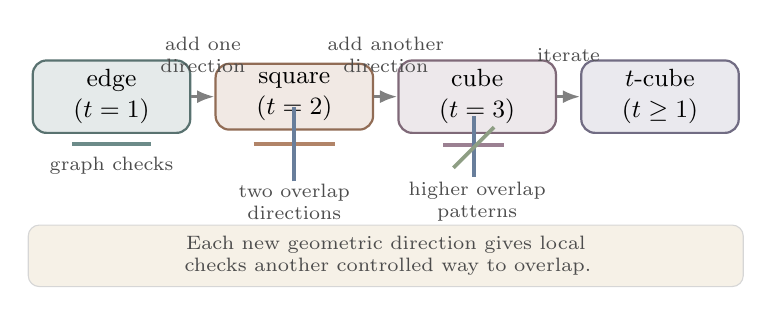
\begin{tikzpicture}[
  scale=0.86,
  every node/.style={font=\small},
  stepbox/.style={draw=#1!82!black,fill=#1!18,rounded corners=5pt,minimum width=2.0cm,minimum height=0.58cm,line width=0.8pt,align=center},
  arrow/.style={-{Latex[length=2.2mm]},line width=1.0pt,draw=black!50},
  note/.style={font=\scriptsize,align=center,text=black!70}
]
  \node[stepbox=morandiTeal]     (e) at (0,0) {edge\\$(t=1)$};
  \node[stepbox=morandiClay]     (s) at (2.7,0) {square\\$(t=2)$};
  \node[stepbox=morandiMauve]    (c) at (5.4,0) {cube\\$(t=3)$};
  \node[stepbox=morandiLavender] (h) at (8.1,0) {$t$-cube\\$(t\ge 1)$};

  \draw[arrow] (e) -- (s);
  \draw[arrow] (s) -- (c);
  \draw[arrow] (c) -- (h);
  \node[note] at (1.35,0.62) {add one\\direction};
  \node[note] at (4.05,0.62) {add another\\direction};
  \node[note] at (6.75,0.62) {iterate};

  \draw[morandiTeal,line width=1.4pt] (-0.58,-0.7) -- (0.58,-0.7);
  \node[note] at (0,-1.02) {graph checks};

  \draw[morandiClay,line width=1.4pt] (2.1,-0.7) -- (3.3,-0.7);
  \draw[morandiBlue,line width=1.4pt] (2.7,-1.25) -- (2.7,-0.15);
  \node[note] at (2.7,-1.55) {two overlap\\directions};

  \draw[morandiMauve,line width=1.4pt] (4.9,-0.72) -- (5.8,-0.72);
  \draw[morandiBlue,line width=1.4pt] (5.35,-1.18) -- (5.35,-0.28);
  \draw[morandiSage,line width=1.4pt] (5.05,-1.05) -- (5.65,-0.45);
  \node[note] at (5.4,-1.55) {higher overlap\\patterns};

  \node[draw=black!16,fill=morandiCream,rounded corners=4pt,inner sep=4pt,note,text width=8.8cm]
    at (4.05,-2.35)
    {Each new geometric direction gives local checks another controlled way to overlap.};
\end{tikzpicture}
\end{center}
\caption{The geometric ladder behind the subject. The muted directions emphasize that the code-theoretic point is not the cell shape itself, but the increasingly rich way local constraints overlap.}
\end{figure}
\textbf{1. The one-dimensional model: expander codes.}

The classical starting point is a \emph{Tanner code} on a sparse expanding graph. \emph{Expansion} is the mechanism that turns local violations into global detectability.

\begin{definition}[Tanner code~\cite{Tanner1981}]
Let $\Gamma=(L,R,E)$ be a bipartite graph, and assume every right vertex has degree $d$. Think of $L$ as the set of \emph{variables} and $R$ as the set of \emph{local constraints}. Fix a linear code $C_0\subseteq \mathbb F_q^d$, called the \emph{local code} or \emph{constraint code}. For each $r\in R$, choose an ordering
\[
\iota_r:N(r)\xrightarrow{\sim}[d].
\]
The associated Tanner code is
\[
C(\Gamma,C_0):=\Bigl\{x\in \mathbb F_q^L:\bigl(x_v\bigr)_{v\in N(r)}\circ \iota_r^{-1}\in C_0\ \text{for every }r\in R\Bigr\}.
\]
Thus a word is accepted exactly when every \emph{local view} around a constraint vertex belongs to the same local code $C_0$.
\end{definition}

\begin{definition}[Sipser--Spielman expander code~\cite{SS}]
Let $\Gamma=(V,E)$ be a finite $d$-regular graph, usually taken from a family of bounded-degree expanders. Fix a linear \emph{short local code}
\[
C_0\subseteq \mathbb F_q^d.
\]
Here \emph{short} means that the block length $d$ is the degree of the graph, usually a fixed constant independent of $|V|$; the same constraint code $C_0$ is reused at every vertex.
For each vertex $v\in V$, choose an ordering of the incident edges
\[
\iota_v:E(v)\xrightarrow{\sim}[d],
\qquad E(v):=\{e\in E:v\in e\}.
\]
The Sipser--Spielman expander code associated to $(\Gamma,C_0)$ is the edge-labeling code
\[
C_{\mathrm{SS}}(\Gamma,C_0):=
\Bigl\{x\in \mathbb F_q^E:
\bigl(x_e\bigr)_{e\in E(v)}\circ \iota_v^{-1}\in C_0
\ \text{for every }v\in V\Bigr\}.
\]
Equivalently, each vertex sees the $d$ symbols on its incident edges and checks that this \emph{length-$d$ local word} lies in $C_0$. The \emph{expansion} of $\Gamma$ is what prevents many small local errors from remaining globally invisible: a small set of corrupted edge symbols has many boundary vertices, and hence creates many violated local constraints.~\cite{SS}
\end{definition}

\begin{figure}[h]
\centering
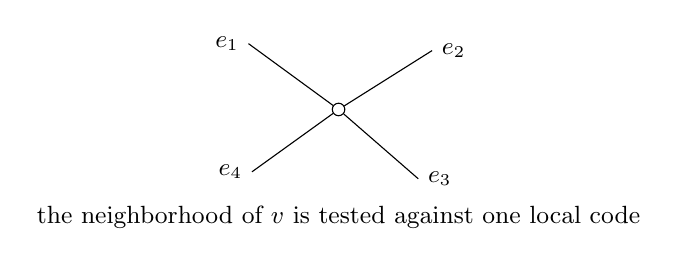
\begin{tikzpicture}[scale=0.88, every node/.style={font=\small}]
  \node[circle,draw,inner sep=1.6pt,fill=white] (v) at (0,0) {};
  \draw (v) -- (-1.3,0.95) node[left] {$e_1$};
  \draw (v) -- (1.35,0.85) node[right] {$e_2$};
  \draw (v) -- (1.15,-1.0) node[right] {$e_3$};
  \draw (v) -- (-1.25,-0.9) node[left] {$e_4$};
  \node at (0,-1.55) {the neighborhood of $v$ is tested against one local code};
\end{tikzpicture}
\caption{One-dimensional local-to-global propagation. The star around a vertex is the local test domain. Expansion forces a small corrupted set to hit many checks.}
\end{figure}

\textbf{2. The first-dimensional lift: left-right Cayley square complexes.}

The two-dimensional analogue replaces an \emph{edge} by a \emph{square} and a star by an $A\times B$ array of incident squares. This is the geometry introduced by Dinur--Evra--Livne--Lubotzky--Mozes.~\cite{DELLM}

\begin{definition}[Left-right Cayley complex]
Let $G$ be a finite group and let $A=A^{-1}$ and $B=B^{-1}$ be symmetric generating sets. The left-right Cayley complex
\[
\mathrm{Cay}_2(A,G,B)
\]
has:
\begin{itemize}
\item vertices $X^{(0)}=G$;
\item $A$-edges and $B$-edges
\[
X_A^{(1)}=\bigl\{\{g,ag\}:g\in G,\ a\in A\bigr\},\qquad
X_B^{(1)}=\bigl\{\{g,gb\}:g\in G,\ b\in B\bigr\};
\]
\item squares indexed by labeled triples $(a,g,b)\in A\times G\times B$:
\[
X^{(2)}=\bigl\{[a,g,b]:g\in G,\ a\in A,\ b\in B\bigr\},
\]
where the square $[a,g,b]$ is the combinatorial face with vertex set $\{g,ag,gb,agb\}$.
\end{itemize}
Note that distinct labeled triples may share the same vertex set (e.g., $[a,g,b]$ and $[a^{-1},ag,b]$ have identical vertices), so the face $[a,g,b]$ must be understood as the labeled cell $(a,g,b)$, not merely its vertex set.
The notation is justified by the commuting left/right actions: $a(gb)=(ag)b$.~\cite{DELLM}
\end{definition}

\begin{figure}[h]
\begin{center}
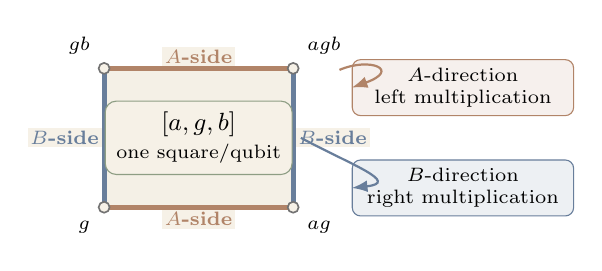
\begin{tikzpicture}[
  scale=0.98,
  every node/.style={font=\small},
  vtx/.style={circle,draw=black!55,fill=morandiCream,inner sep=1.4pt,line width=0.6pt},
  alabel/.style={font=\scriptsize\bfseries,text=morandiClay,fill=morandiCream,inner sep=1pt},
  blabel/.style={font=\scriptsize\bfseries,text=morandiBlue,fill=morandiCream,inner sep=1pt},
  calloutA/.style={draw=morandiClay,fill=morandiClay!12,rounded corners=3pt,inner sep=3pt,align=center,font=\scriptsize},
  calloutB/.style={draw=morandiBlue,fill=morandiBlue!12,rounded corners=3pt,inner sep=3pt,align=center,font=\scriptsize}
]
  \coordinate (g) at (0,0);
  \coordinate (ag) at (2.45,0);
  \coordinate (gb) at (0,1.8);
  \coordinate (agb) at (2.45,1.8);

  \fill[morandiSand!35,rounded corners=4pt] (g) rectangle (agb);
  \draw[morandiClay,line width=1.8pt] (g) -- node[below,alabel] {$A$-side} (ag);
  \draw[morandiClay,line width=1.8pt] (gb) -- node[above,alabel] {$A$-side} (agb);
  \draw[morandiBlue,line width=1.8pt] (g) -- node[left,blabel] {$B$-side} (gb);
  \draw[morandiBlue,line width=1.8pt] (ag) -- node[right,blabel] {$B$-side} (agb);

  \node[vtx,label={[font=\scriptsize]below left:$g$}] at (g) {};
  \node[vtx,label={[font=\scriptsize]below right:$ag$}] at (ag) {};
  \node[vtx,label={[font=\scriptsize]above left:$gb$}] at (gb) {};
  \node[vtx,label={[font=\scriptsize]above right:$agb$}] at (agb) {};

  \node[draw=morandiSage,fill=morandiCream,rounded corners=4pt,inner sep=4pt,align=center]
    at (1.225,0.9) {$[a,g,b]$\\[-1pt]\scriptsize one square/qubit};

  \node[calloutA,text width=2.6cm] (Abox) at (4.65,1.55) {$A$-direction\\left multiplication};
  \node[calloutB,text width=2.6cm] (Bbox) at (4.65,0.25) {$B$-direction\\right multiplication};

  \draw[-{Latex[length=2mm]},draw=morandiClay,line width=0.8pt]
    (3.05,1.78) .. controls (3.45,1.95) and (3.85,1.78) .. (Abox.west);
  \draw[-{Latex[length=2mm]},draw=morandiBlue,line width=0.8pt]
    (2.55,0.9) .. controls (3.2,0.55) and (3.85,0.32) .. (Bbox.west);
\end{tikzpicture}
\end{center}
\caption{A canonical square in the left-right Cayley complex. Muted clay sides mark the $A$-direction and muted blue sides mark the $B$-direction; the controlled overlap of these two directions is the key new ingredient absent from graph-based codes.}
\end{figure}

The local view around a vertex is naturally a \emph{tensor-code neighborhood}.

\begin{definition}[Tensor product code]
Let $C_A\subseteq \mathbb F_q^A$ and $C_B\subseteq \mathbb F_q^B$ be linear codes. Their tensor product is
\[
C_A\otimes C_B:=\Bigl\{M\in \mathbb F_q^{A\times B}: M(a,\cdot)\in C_B\ \forall a\in A,\ \ M(\cdot,b)\in C_A\ \forall b\in B\Bigr\}.
\]
Equivalently, every \emph{row} lies in $C_B$ and every \emph{column} lies in $C_A$. (This is a classical construction; the presentation here follows~\cite{DELLM}.)
\end{definition}

\begin{figure}[h]
\begin{center}
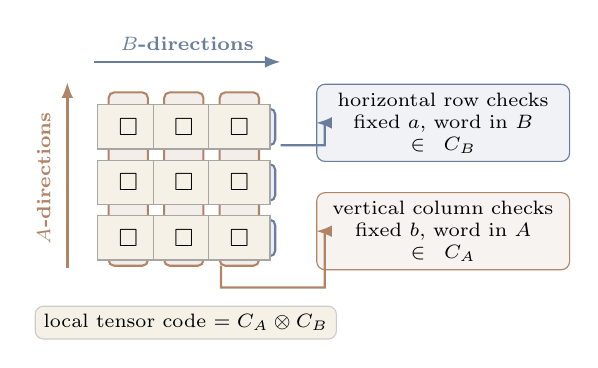
\begin{tikzpicture}[
  scale=0.86,
  every node/.style={font=\small},
  cell/.style={draw=black!35,fill=morandiCream,minimum width=0.78cm,minimum height=0.56cm,inner sep=0pt},
  rowcheck/.style={draw=morandiBlue,fill=morandiBlue!14,rounded corners=2pt,line width=0.75pt},
  colcheck/.style={draw=morandiClay,fill=morandiClay!14,rounded corners=2pt,line width=0.75pt},
  calloutRow/.style={draw=morandiBlue,fill=morandiBlue!10,rounded corners=3pt,inner sep=3pt,align=center,font=\scriptsize,text width=3.0cm},
  calloutCol/.style={draw=morandiClay,fill=morandiClay!10,rounded corners=3pt,inner sep=3pt,align=center,font=\scriptsize,text width=3.0cm}
]
  % Row and column check bands, deliberately muted.
  \foreach \j in {0,1,2} {
    \draw[rowcheck] (-0.06,{0.08+0.82*\j}) rectangle (2.52,{0.62+0.82*\j});
  }
  \foreach \i in {0,1,2} {
    \draw[colcheck] ({0.06+0.82*\i},-0.06) rectangle ({0.64+0.82*\i},2.50);
  }

  % Cells / qubits.
  \foreach \i in {0,1,2} {
    \foreach \j in {0,1,2} {
      \node[cell] at ({0.35+0.82*\i},{0.35+0.82*\j}) {$\square$};
    }
  }

  % Axes and labels.
  \draw[-{Latex[length=2mm]},line width=0.85pt,draw=morandiBlue] (-0.15,2.95) -- (2.6,2.95);
  \node[text=morandiBlue,font=\scriptsize\bfseries] at (1.22,3.22) {$B$-directions};

  \draw[-{Latex[length=2mm]},line width=0.85pt,draw=morandiClay] (-0.55,-0.1) -- (-0.55,2.65);
  \node[rotate=90,text=morandiClay,font=\scriptsize\bfseries] at (-0.9,1.23) {$A$-directions};

  \node[calloutRow] (rowbox) at (5.0,2.05) {horizontal row checks\\fixed $a$, word in $B$\\$\in C_B$};
  \node[calloutCol] (colbox) at (5.0,0.45) {vertical column checks\\fixed $b$, word in $A$\\$\in C_A$};

  % Route arrows cleanly into the left edges of the callout boxes.
  \draw[-{Latex[length=2mm]},draw=morandiBlue,line width=0.8pt]
    (2.60,1.72) -- (3.25,1.72) -- (3.25,2.05) -- (rowbox.west);
  \draw[-{Latex[length=2mm]},draw=morandiClay,line width=0.8pt]
    (1.72,-0.06) -- (1.72,-0.38) -- (3.25,-0.38) -- (3.25,0.45) -- (colbox.west);

  \node[draw=black!20,fill=morandiCream,rounded corners=3pt,inner sep=3pt,align=center,font=\scriptsize]
    at (1.2,-0.9) {local tensor code $=C_A\otimes C_B$};
\end{tikzpicture}
\end{center}
\caption{The squares incident to a vertex form an $A\times B$ array. Muted blue horizontal bands show the row checks, while muted clay vertical bands show the column checks. In the convention above, rows are words in $C_B$ and columns are words in $C_A$.}
\end{figure}

\begin{definition}[Quantum Tanner code]
Let $\widetilde X$ be the bipartite-covered left-right Cayley complex with vertex set
\[
V_{ij}=G\times\{(i,j)\},\qquad i,j\in\{0,1\},
\]
and with faces inherited from the left-right squares. Fix classical codes $C_A\subseteq \mathbb F_2^A$ and $C_B\subseteq \mathbb F_2^B$. A quantum Tanner code is the CSS code with
\begin{itemize}
\item qubits on the faces of $\widetilde X$;
\item $X$-checks at vertices $V_0:=V_{00}\sqcup V_{11}$, where the local check space on the incident faces $Q(v)\cong A\times B$ is $C_A\otimes C_B$;
\item $Z$-checks at vertices $V_1:=V_{01}\sqcup V_{10}$, where the local check space on $Q(v)$ is $C_A^{\perp}\otimes C_B^{\perp}$.
\end{itemize}
The CSS condition $H_X H_Z^T = 0$ is verified by direct face incidence. A face $[a,g,b]$ in the bipartite cover has four vertices: $(g,00),(ag,10),(gb,01),(agb,11)$. An $X$-check at $v=(g,00)\in V_{00}$ is supported on all faces incident to $v$, namely $Q(v)=\{[a,g,b]:a\in A,b\in B\}$, and defines a vector $u\in C_A\otimes C_B$. A $Z$-check at $w=(gb_0,01)\in V_{01}$ is supported on $Q(w)=\{[a,g',b']: g'b'=gb_0,\,a\in A,b'\in B\}$, and defines $v'\in C_A^\perp\otimes C_B^\perp$. A face $[a,g,b]$ lies in $Q(v)\cap Q(w)$ iff $gb=gb_0$, i.e., $b=b_0$. Thus $Q(v)\cap Q(w)=\{[a,g,b_0]:a\in A\}$, a single column of the $A\times B$ array. On this column, $u(\cdot,b_0)\in C_A$ and $v'(\cdot,b_0)\in C_A^\perp$, so $\langle u(\cdot,b_0),v'(\cdot,b_0)\rangle=0$. An analogous argument covers the $(V_{00},V_{10})$, $(V_{11},V_{01})$, and $(V_{11},V_{10})$ pairs, in each case reducing the overlap to a single row or column and applying $C_A\perp C_A^\perp$ or $C_B\perp C_B^\perp$. If the underlying degrees are bounded, the family is qLDPC.~\cite{QT}
\end{definition}


\begin{figure}[h]
\centering
\resizebox{\linewidth}{!}{%
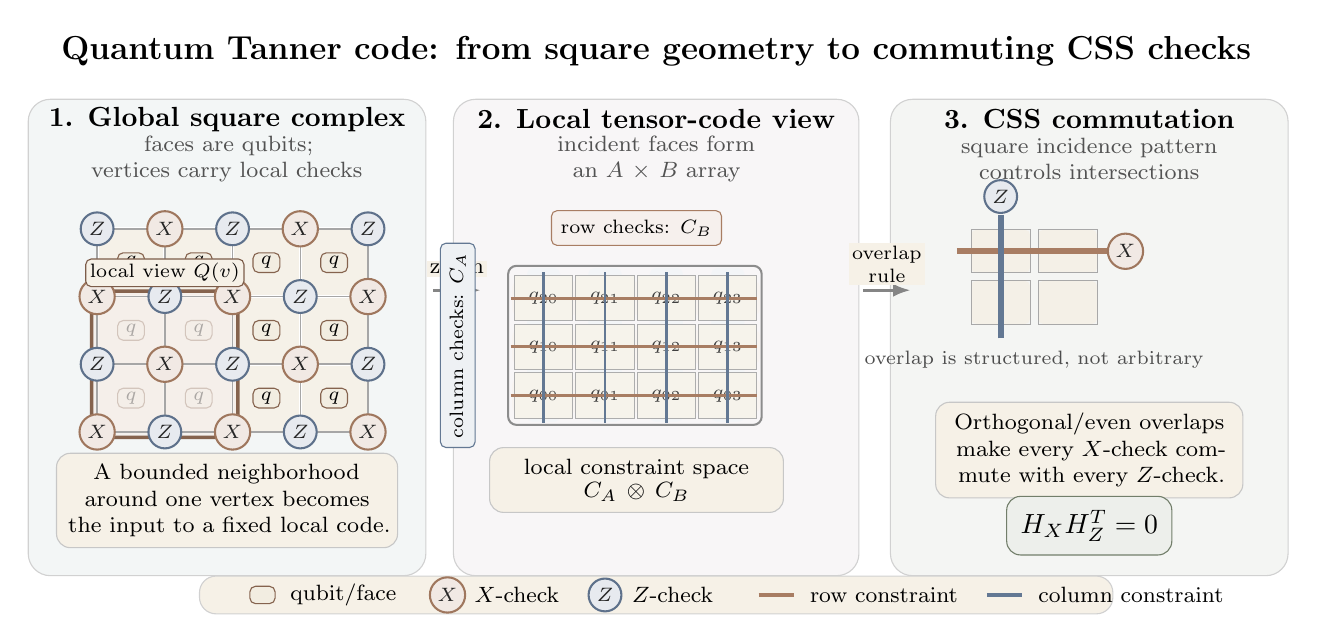
\begin{tikzpicture}[
  font=\small,
  >=Latex,
  panel/.style={draw=black!18,rounded corners=8pt,fill=#1,inner sep=0pt},
  title/.style={font=\bfseries\large,align=center},
  subtitle/.style={font=\footnotesize,align=center,text=black!68},
  qubit/.style={draw=morandiClay!75!black,fill=morandiSand!42,rounded corners=2pt,minimum width=0.48cm,minimum height=0.34cm,inner sep=1pt,font=\scriptsize},
  xcheck/.style={circle,draw=morandiClay!90!black,fill=morandiClay!18,line width=0.75pt,inner sep=1.5pt,font=\scriptsize\bfseries,text=black!85},
  zcheck/.style={circle,draw=morandiBlue!90!black,fill=morandiBlue!16,line width=0.75pt,inner sep=1.5pt,font=\scriptsize\bfseries,text=black!85},
  callout/.style={draw=black!22,rounded corners=5pt,fill=morandiCream,align=center,inner sep=4pt,font=\footnotesize},
  flowarrow/.style={-{Latex[length=2.2mm]},line width=1.05pt,draw=black!48},
  rowband/.style={draw=morandiClay!95!black,fill=morandiClay!12,rounded corners=2pt},
  colband/.style={draw=morandiBlue!95!black,fill=morandiBlue!11,rounded corners=2pt}
]

% Muted Morandi panels
\node[panel=morandiTeal!8,minimum width=5.05cm,minimum height=6.05cm] at (2.3,2.55) {};
\node[panel=morandiMauve!7,minimum width=5.15cm,minimum height=6.05cm] at (7.75,2.55) {};
\node[panel=morandiSage!10,minimum width=5.05cm,minimum height=6.05cm] at (13.25,2.55) {};

\node[title] at (7.75,6.18) {Quantum Tanner code: from square geometry to commuting CSS checks};

% Panel 1: global complex
\node[font=\bfseries\normalsize] at (2.3,5.32) {1. Global square complex};
\node[subtitle,text width=3.65cm] at (2.3,4.82) {faces are qubits;\\ vertices carry local checks};
\begin{scope}[shift={(0.65,1.35)},scale=0.86]
  % faces
  \foreach \x in {0,1,2,3}{
    \foreach \y in {0,1,2}{
      \fill[morandiSand!32] (\x,\y) rectangle +(1,1);
      \draw[white,line width=1.0pt] (\x,\y) rectangle +(1,1);
      \node[qubit,minimum width=0.34cm,minimum height=0.25cm] at (\x+0.5,\y+0.5) {$q$};
    }
  }
  % local neighborhood highlight goes behind checks, but after cells
  \fill[morandiClay!13,opacity=0.70,rounded corners=4pt] (-0.08,-0.08) rectangle (2.08,2.08);
  \draw[morandiClay!75!black,line width=1.25pt,rounded corners=4pt] (-0.08,-0.08) rectangle (2.08,2.08);
  % grid lines
  \foreach \x in {0,1,2,3,4}{\draw[black!35,line width=0.55pt] (\x,0)--(\x,3);}
  \foreach \y in {0,1,2,3}{\draw[black!35,line width=0.55pt] (0,\y)--(4,\y);}
  % checks
  \foreach \x in {0,1,2,3,4}{
    \foreach \y in {0,1,2,3}{
      \pgfmathtruncatemacro{\parity}{mod(\x+\y,2)}
      \ifnum\parity=0
        \node[xcheck] at (\x,\y) {$X$};
      \else
        \node[zcheck] at (\x,\y) {$Z$};
      \fi
    }
  }
  % label above the highlight, not intersecting arrows
  \node[font=\scriptsize,fill=morandiCream,draw=morandiClay!70!black,rounded corners=2pt,inner sep=1.5pt] at (1,2.35) {local view $Q(v)$};
\end{scope}
\node[callout,text width=4.05cm] at (2.3,0.48) {A bounded neighborhood around one vertex becomes the input to a fixed local code.};

% Flow arrow 1 in the gutter; no overlap with callout boxes
\draw[flowarrow] (4.92,3.15) -- (5.52,3.15);
\node[font=\footnotesize,fill=morandiCream,inner sep=1.2pt] at (5.22,3.42) {zoom};

% Panel 2: local tensor view
\node[font=\bfseries\normalsize] at (7.75,5.32) {2. Local tensor-code view};
\node[subtitle,text width=3.75cm] at (7.75,4.82) {incident faces form\\ an $A\times B$ array};
\begin{scope}[shift={(5.95,1.52)}]
  % background soft row and column bands, separated from labels
  \foreach \j in {0,1,2}{
    \fill[morandiClay!9,rounded corners=2pt] (-0.03,0.62*\j+0.08) rectangle (3.12,0.62*\j+0.50);
  }
  \foreach \i in {0,1,2,3}{
    \fill[morandiBlue!8,rounded corners=2pt] (0.78*\i+0.16,-0.04) rectangle (0.78*\i+0.58,1.91);
  }
  \foreach \i in {0,1,2,3}{
    \foreach \j in {0,1,2}{
      \fill[morandiSand!28] (0.78*\i,0.62*\j) rectangle +(0.74,0.58);
      \draw[black!32,line width=0.35pt] (0.78*\i,0.62*\j) rectangle +(0.74,0.58);
      \node[font=\scriptsize,text=black!75] at (0.78*\i+0.37,0.62*\j+0.29) {$q_{\j\i}$};
    }
  }
  % row and column constraint strokes
  \foreach \j in {0,1,2}{
    \draw[morandiClay!95!black,line width=1.05pt] (-0.05,0.62*\j+0.29) -- (3.08,0.62*\j+0.29);
  }
  \foreach \i in {0,1,2,3}{
    \draw[morandiBlue!95!black,line width=1.05pt] (0.78*\i+0.37,-0.05) -- (0.78*\i+0.37,1.86);
  }
  \draw[black!45,rounded corners=3pt,line width=0.75pt] (-0.08,-0.08) rectangle (3.14,1.94);
  \node[rowband,minimum width=1.75cm,minimum height=0.38cm,font=\scriptsize] at (1.55,2.42) {row checks: $C_B$};
  \node[colband,minimum width=1.85cm,minimum height=0.38cm,font=\scriptsize,rotate=90] at (-0.72,0.93) {column checks: $C_A$};
  \node[callout,text width=3.45cm] at (1.55,-0.78) {local constraint space\\[-1pt] $C_A\otimes C_B$};
\end{scope}

% Flow arrow 2 above the lower callout and below panel title, routed through empty gutter
\draw[flowarrow] (10.38,3.15) -- (10.98,3.15);
\node[font=\scriptsize,fill=morandiCream,inner sep=1.2pt,align=center] at (10.68,3.48) {overlap\\rule};

% Panel 3: CSS commutation
\node[font=\bfseries\normalsize] at (13.25,5.32) {3. CSS commutation};
\node[subtitle,text width=3.7cm] at (13.25,4.82) {square incidence pattern\\ controls intersections};
\begin{scope}[shift={(11.75,2.72)}]
  % overlap cartoon
  \foreach \x/\y in {0/0,0.85/0,0/0.65,0.85/0.65}{
    \fill[morandiSand!34,rounded corners=2pt] (\x,\y) rectangle +(0.75,0.55);
    \draw[black!34] (\x,\y) rectangle +(0.75,0.55);
  }
  \draw[morandiClay!95!black,line width=2.2pt,rounded corners=8pt] (-0.18,0.925) -- (1.78,0.925);
  \draw[morandiBlue!95!black,line width=2.2pt,rounded corners=8pt] (0.375,-0.18) -- (0.375,1.38);
  \node[xcheck] at (1.96,0.925) {$X$};
  \node[zcheck] at (0.375,1.62) {$Z$};
  \node[font=\scriptsize,text=black!70] at (0.80,-0.45) {overlap is structured, not arbitrary};
\end{scope}
\node[callout,text width=3.62cm] at (13.25,1.12) {Orthogonal/even overlaps make every $X$-check commute with every $Z$-check.};
\node[draw=morandiSage!80!black,fill=morandiSage!16,rounded corners=5pt,inner sep=5pt,font=\bfseries] at (13.25,0.16) {$H_XH_Z^T=0$};

% Legend strip
\node[draw=black!18,fill=morandiCream,rounded corners=6pt,minimum width=11.6cm,minimum height=0.48cm] at (7.75,-0.72) {};
\node[qubit,minimum width=0.32cm,minimum height=0.22cm] at (2.75,-0.72) {};
\node[anchor=west,font=\footnotesize] at (2.98,-0.72) {qubit/face};
\node[xcheck] at (5.10,-0.72) {$X$};
\node[anchor=west,font=\footnotesize] at (5.32,-0.72) {$X$-check};
\node[zcheck] at (7.10,-0.72) {$Z$};
\node[anchor=west,font=\footnotesize] at (7.32,-0.72) {$Z$-check};
\draw[morandiClay!95!black,line width=1.5pt] (9.05,-0.72)--(9.50,-0.72);
\node[anchor=west,font=\footnotesize] at (9.58,-0.72) {row constraint};
\draw[morandiBlue!95!black,line width=1.5pt] (11.95,-0.72)--(12.40,-0.72);
\node[anchor=west,font=\footnotesize] at (12.48,-0.72) {column constraint};

\end{tikzpicture}%
}
\caption{A more visual picture of a quantum Tanner code.  The left panel shows the global square complex: qubits sit on faces and the two vertex types support $X$- and $Z$-checks.  The middle panel zooms into one vertex, where the incident faces form an $A\times B$ tensor neighborhood carrying the local constraint $C_A\otimes C_B$.  Here, rows (horizontal, fixing $a\in A$) are checked against $C_B$, and columns (vertical, fixing $b\in B$) are checked against $C_A$, consistent with the definition $M(a,\cdot)\in C_B$ and $M(\cdot,b)\in C_A$.  The right panel shows the key CSS point: the square-complex incidence pattern makes $X$-$Z$ overlaps controlled, giving $H_XH_Z^T=0$.  Note that this figure uses the square-complex orientation in which $A$-edges run horizontally and $B$-edges run vertically, which is the transpose of the standalone tensor-product figure above.}
\label{fig:quantum-tanner-visual}
\end{figure}



\begin{definition}[qLDPC and qLTC, CSS form]
A CSS code with parity-check matrices $H_X,H_Z$ is \emph{qLDPC} if the row and column weights of both matrices are uniformly bounded. It is a \emph{qLTC} with soundness $\rho>0$ if, for every Pauli error $E = X^{e_X}Z^{e_Z}$ with $e_X,e_Z\in\mathbb F_2^n$, the total syndrome weight
\[
|\mathrm{synd}(E)| \;:=\; |H_X e_Z| + |H_Z e_X|
\]
satisfies $|\mathrm{synd}(E)| \ge \rho\cdot \mathrm{wt}_{\mathrm{corr}}(E)$, where $\mathrm{wt}_{\mathrm{corr}}(E):=\min_{s\in S}\mathrm{wt}(sE)$ is the minimum qubit weight of any Pauli correction of $E$ to the codespace (i.e., the distance of the error coset to the identity). For CSS codes, a \emph{sufficient} condition---employed throughout the chain-complex framework---is that both classical codes $\ker H_X$ and $\ker H_Z$ are individually locally testable with constant soundness; the quantum soundness constant is then bounded below in terms of the two classical constants.~\cite{DLV,WLH}
\end{definition}


\textbf{3. Stabilizer codes: two concrete examples.}

Before returning to higher cubical complexes, it is useful to isolate three basic notions that recur later: 
\emph{stabilizers}, \emph{logical operators}, and \emph{logical sectors}.  These notions are standard in the stabilizer formalism~\cite{Gottesman1997}, but they also have a geometric interpretation in CSS codes~\cite{CS1996}: in codes arising from chain complexes, stabilizers are local boundaries or coboundaries, logical operators are global cycles not generated locally, and logical sectors are the resulting encoded degrees of freedom.~\cite{Kitaev2003}


Intuitively, a Pauli operator is a basic \emph{bit-flip} or \emph{phase-flip} operation on one or more qubits. The operator $X$ flips $|0\rangle$ and $|1\rangle$,
\[
X|0\rangle=|1\rangle,
\qquad
X|1\rangle=|0\rangle,
\]
while $Z$ leaves $|0\rangle$ fixed and changes the sign of $|1\rangle$,
\[
Z|0\rangle=|0\rangle,
\qquad
Z|1\rangle=-|1\rangle.
\]
Multi-qubit Pauli operators are tensor products of these single-qubit operations. For instance,
\[
X_1Z_3X_5
=
X\otimes I\otimes Z\otimes I\otimes X.
\]
The key feature is that Pauli operators either \emph{commute} or \emph{anticommute}. On one qubit,
\[
XZ=-ZX,
\]
but operators acting on different qubits commute. Thus two multi-qubit Pauli operators commute precisely when the number of qubits on which they anticommute is even. In a stabilizer code, the stabilizers are chosen to commute, so they can be imposed as compatible quantum parity checks.

A stabilizer is therefore a check that every valid code state must pass. Passing the check $s$ means being fixed by it:
\[
s|\psi\rangle=|\psi\rangle.
\]
Thus the code space is the simultaneous $+1$ eigenspace of all stabilizers: it consists exactly of the states that are fixed by every stabilizer operator.

Let $\mathcal P_n$ denote the $n$-qubit Pauli group, generated by the single-qubit Pauli operators $X_i,Z_i$ together with phases.

\begin{definition}[Stabilizers]
A \emph{stabilizer group} on $n$ qubits is an abelian subgroup
\[
S\subseteq \mathcal P_n
\]
such that $-I\notin S$. The associated quantum code space is the common $+1$ eigenspace
\[
\mathcal C(S):=
\{\,|\psi\rangle\in (\mathbb C^2)^{\otimes n}:
 s|\psi\rangle=|\psi\rangle\text{ for every }s\in S\,\}.
\]
Elements of $S$ are called \emph{stabilizers}. They are the quantum analogue of parity checks: they impose local constraints that every valid code state must satisfy.

For a CSS code with parity-check matrices $H_X,H_Z$, the stabilizers are generated by the rows of $H_X$ and $H_Z$: a row of $H_X$ gives an $X$-type Pauli check, and a row of $H_Z$ gives a $Z$-type Pauli check. The CSS commutation condition is
\[
H_XH_Z^T=0.
\]
\end{definition}

\begin{definition}[Logical operators]
The \emph{normalizer} of the stabilizer group is
\[
N(S):=
\{\,p\in \mathcal P_n: ps=sp\text{ for every }s\in S\,\}.
\]
A Pauli operator $p\in N(S)$ preserves the code space because it commutes with every stabilizer. Operators in $S$ act trivially on the code space, so the nontrivial logical Pauli operators are the elements of the quotient
\[
\overline{\mathcal P}:=N(S)/S.
\]
Thus a \emph{logical operator} is a Pauli operator that preserves the code space but is not equivalent, on the code space, to a product of stabilizers. Equivalently, logical operators are the physical Pauli operators that act nontrivially on the encoded qubits.

In CSS notation, the $X$-type and $Z$-type logical operators are represented by the quotient spaces
\[
\ker H_Z\big/\operatorname{im}(H_X^T),
\qquad
\ker H_X\big/\operatorname{im}(H_Z^T).
\]
The numerator says ``commutes with the opposite checks,'' while the denominator says ``mod out by products of stabilizers.''
\end{definition}

\begin{definition}[Logical sectors]
Suppose the code encodes $k$ logical qubits, so that
\[
\dim \mathcal C(S)=2^k.
\]
Choose representatives of logical Pauli operators
\[
\overline Z_1,\dots,\overline Z_k,
\qquad
\overline X_1,\dots,\overline X_k,
\]
satisfying the usual Pauli commutation relations on the code space. The \emph{logical sectors} with respect to the chosen logical $Z$-basis are the simultaneous eigenspaces
\[
\mathcal C_{\mathbf a}:=
\{\,|\psi\rangle\in \mathcal C(S):
\overline Z_i|\psi\rangle=(-1)^{a_i}|\psi\rangle
\text{ for }i=1,\dots,k\,\},
\qquad
\mathbf a=(a_1,\dots,a_k)\in \mathbb F_2^k.
\]
Thus the stabilizers define the code space, while the logical sectors label the different encoded basis states inside that code space.

In many homological or geometric CSS codes, logical sectors can be viewed as \emph{homology classes}: two representatives describe the same logical sector if they differ by a product of local stabilizers.
\end{definition}

\begin{figure}[h]
\centering
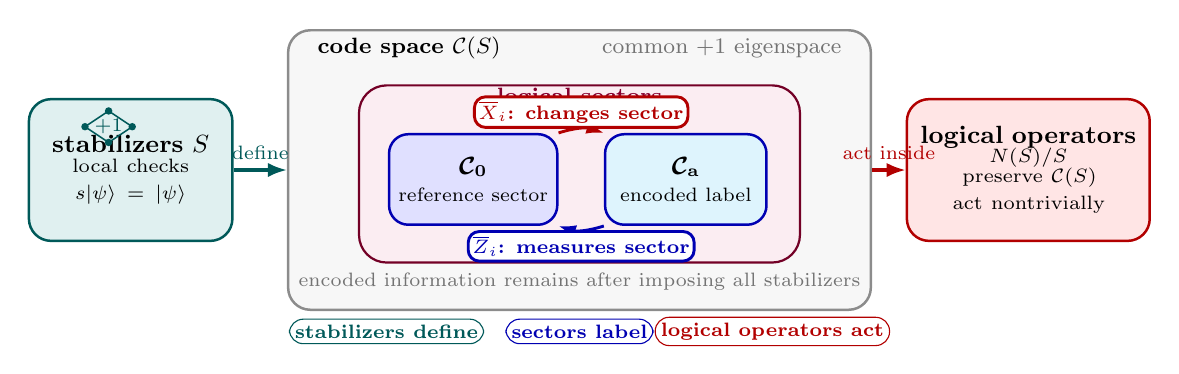
\begin{tikzpicture}[x=1cm,y=1cm,every node/.style={font=\small}]
  % Outer code space
  \node[
    draw=black!45,
    fill=gray!6,
    line width=0.9pt,
    rounded corners=8pt,
    minimum width=7.4cm,
    minimum height=3.55cm
  ] (code) at (0,0) {};
  \node[anchor=west,font=\footnotesize\bfseries] at (-3.45,1.55)
    {code space $\mathcal C(S)$};
  \node[anchor=east,font=\footnotesize,text=black!55] at (3.45,1.55)
    {common $+1$ eigenspace};

  % Logical-sector band
  \node[
    draw=purple!60!black,
    fill=purple!7,
    line width=0.8pt,
    rounded corners=10pt,
    minimum width=5.6cm,
    minimum height=2.25cm
  ] (band) at (0,-0.05) {};
  \node[font=\footnotesize\bfseries,text=purple!70!black] at (0,0.92)
    {logical sectors};

  % Logical sectors
  \node[
    draw=blue!70!black,
    fill=blue!12,
    line width=0.9pt,
    rounded corners=7pt,
    minimum width=2.05cm,
    minimum height=1.15cm,
    align=center
  ] (sector0) at (-1.35,-0.12)
    {$\boldsymbol{\mathcal C_{\mathbf 0}}$\\[-1pt]
     \scriptsize reference sector};

  \node[
    draw=blue!70!black,
    fill=cyan!13,
    line width=0.9pt,
    rounded corners=7pt,
    minimum width=2.05cm,
    minimum height=1.15cm,
    align=center
  ] (sectora) at (1.35,-0.12)
    {$\boldsymbol{\mathcal C_{\mathbf a}}$\\[-1pt]
     \scriptsize encoded label};

  % X and Z arrows
  \draw[-{Latex[length=2.2mm]},line width=1.05pt,red!70!black,bend left=18]
    (sector0.north east) to node[above,fill=white,draw=red!70!black,rounded corners=4pt,inner sep=1.6pt,text=red!70!black,font=\scriptsize\bfseries]
    {$\overline X_i$: changes sector} (sectora.north west);

  \draw[-{Latex[length=2.2mm]},line width=1.05pt,blue!70!black,bend left=18]
    (sectora.south west) to node[below,fill=white,draw=blue!70!black,rounded corners=4pt,inner sep=1.6pt,text=blue!70!black,font=\scriptsize\bfseries]
    {$\overline Z_i$: measures sector} (sector0.south east);

  \node[text=black!55,font=\scriptsize,align=center] at (0,-1.42)
    {encoded information remains after imposing all stabilizers};

  % Stabilizer panel
  \node[
    draw=teal!70!black,
    fill=teal!12,
    line width=0.9pt,
    rounded corners=8pt,
    align=center,
    text width=2.35cm,
    minimum height=1.8cm
  ] (stab) at (-5.7,0)
    {\textbf{stabilizers $S$}\\[-1pt]
     \scriptsize local checks\\[-1pt]
     \scriptsize $s|\psi\rangle=|\psi\rangle$};

  \draw[teal!70!black,line width=0.55pt] (-6.28,0.55)--(-5.98,0.75)--(-5.68,0.55)--(-5.98,0.35)--cycle;
  \foreach \p in {(-6.28,0.55),(-5.98,0.75),(-5.68,0.55),(-5.98,0.35)}
    \fill[teal!70!black] \p circle (1.35pt);
  \node[text=teal!70!black,font=\scriptsize\bfseries] at (-5.98,0.55) {$+1$};

  % Logical operator panel
  \node[
    draw=red!70!black,
    fill=red!10,
    line width=0.9pt,
    rounded corners=8pt,
    align=center,
    text width=2.85cm,
    minimum height=1.8cm
  ] (logic) at (5.7,0)
    {\textbf{logical operators}\\[-1pt]
     \scriptsize $N(S)/S$\\[-1pt]
     \scriptsize preserve $\mathcal C(S)$\\[-1pt]
     \scriptsize act nontrivially};


  % Side arrows
  \draw[-{Latex[length=2.4mm]},line width=1.1pt,teal!70!black]
    (stab.east) -- node[above,font=\scriptsize,text=teal!70!black,align=center]
    {define} (code.west);
  \draw[-{Latex[length=2.4mm]},line width=1.1pt,red!70!black]
    (code.east) -- node[above,font=\scriptsize,text=red!70!black,align=center]
    {act inside} (logic.west);

  % Role legend
  \node[draw=teal!70!black,fill=white,rounded corners=5pt,inner sep=2pt,text=teal!70!black,font=\scriptsize\bfseries]
    at (-2.45,-2.05) {stabilizers define};
  \node[draw=blue!70!black,fill=white,rounded corners=5pt,inner sep=2pt,text=blue!70!black,font=\scriptsize\bfseries]
    at (0,-2.05) {sectors label};
  \node[draw=red!70!black,fill=white,rounded corners=5pt,inner sep=2pt,text=red!70!black,font=\scriptsize\bfseries]
    at (2.45,-2.05) {logical operators act};
\end{tikzpicture}
\caption{Stabilizers, logical operators, and logical sectors. Stabilizers define the code space $\mathcal C(S)$ as a simultaneous $+1$ eigenspace. Logical operators preserve this space but act nontrivially inside it. After choosing a logical basis, the code space decomposes into logical sectors labeled by eigenvalues of the logical $\overline Z_i$ operators.}
\end{figure}


A useful slogan is:
\[
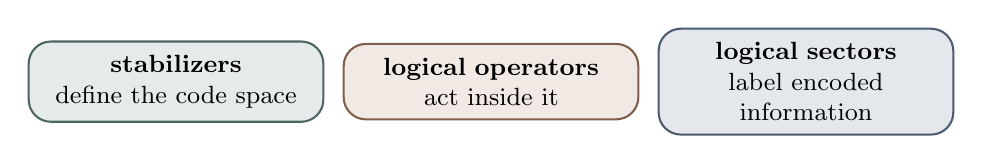
\begin{tikzpicture}[
  baseline=(current bounding box.center),
  every node/.style={font=\small},
  slogan/.style={
    draw=#1!72!black,
    fill=#1!18,
    rounded corners=8pt,
    line width=0.75pt,
    inner xsep=7pt,
    inner ysep=5pt,
    align=center,
    text width=3.25cm
  }
]
  \node[slogan=morandiTeal] (s) at (0,0)
    {\textbf{stabilizers}\\ define the code space};
  \node[slogan=morandiClay] (l) at (4.0,0)
    {\textbf{logical operators}\\ act inside it};
  \node[slogan=morandiBlue] (q) at (8.0,0)
    {\textbf{logical sectors}\\ label encoded information};
\end{tikzpicture}
\]

\textbf{Example 1 (the 3-qubit repetition code).}
Take stabilizer generators
\[
S_1=Z_1Z_2,
\qquad
S_2=Z_2Z_3.
\]
The codespace is
\[
\mathcal C=\operatorname{span}\{|000\rangle,|111\rangle\},
\]
so the code encodes one logical qubit, with logical basis
\[
|0_L\rangle=|000\rangle,
\qquad
|1_L\rangle=|111\rangle.
\]
A standard choice of logical operators is
\[
\overline X=X_1X_2X_3,
\qquad
\overline Z=Z_1,
\]
where any single $Z_i$ serves as an equivalent representative since $Z_1,Z_2,Z_3$ are all equal modulo $S$ (e.g., $Z_2 = Z_1\cdot(Z_1Z_2)\in Z_1\cdot S$). The two logical sectors for the commuting observable $\overline Z$ are therefore the one-dimensional spaces
\[
\operatorname{span}\{|0_L\rangle\}
\quad\text{and}\quad
\operatorname{span}\{|1_L\rangle\}.
\]
This is the smallest example where one can see the hierarchy clearly: \emph{stabilizers} define the codespace, \emph{logical operators} act inside it, and \emph{logical sectors} are eigenspaces inside that codespace.

\textbf{Example 2 (the toric code).}
Place qubits on the edges of an $L\times L$ square lattice with periodic boundary conditions.~\cite{Kitaev2003} For each vertex $v$ and plaquette $p$, define the star and plaquette stabilizers
\[
A_v=\prod_{e\ni v} X_e,
\qquad
B_p=\prod_{e\in \partial p} Z_e.
\]
The global constraints $\prod_v A_v=I$ and $\prod_p B_p=I$ each reduce the rank of the stabilizer generators by one. On the $L\times L$ torus, $|V|=L^2$, $|E|=2L^2$, $|F|=L^2$, and Euler's formula gives $|V|-|E|+|F|=0$, so $n:=|E|=|V|+|F|$. The stabilizer rank is $(|V|-1)+(|F|-1)=|E|-2$, hence $k=n-\operatorname{rank}(S)=|E|-(|E|-2)=2$ encoded logical qubits and four logical sectors. A convenient generating set for the logical operators is given by two noncontractible $Z$-loops $\overline Z_1,\overline Z_2$ around the two fundamental directions of the torus, together with the dual noncontractible $X$-loops $\overline X_1,\overline X_2$, satisfying
\[
\overline X_i\,\overline Z_j=(-1)^{\delta_{ij}}\,\overline Z_j\,\overline X_i.
\]
Thus the codespace decomposes into four sectors labeled by the eigenvalues of $(\overline Z_1,\overline Z_2)$:
\[
(+,+),\quad (+,-),\quad (-,+),\quad (-,-).
\]
Geometrically, \emph{contractible loops} are stabilizers, while \emph{noncontractible loops} are logical operators. This is the topological prototype for the local-to-global viewpoint used throughout the note. Figure~\ref{fig:toric-picture-first} packages the toric-code dictionary in the same picture-first style used elsewhere in the note.

\begin{figure}[!htbp]
\centering
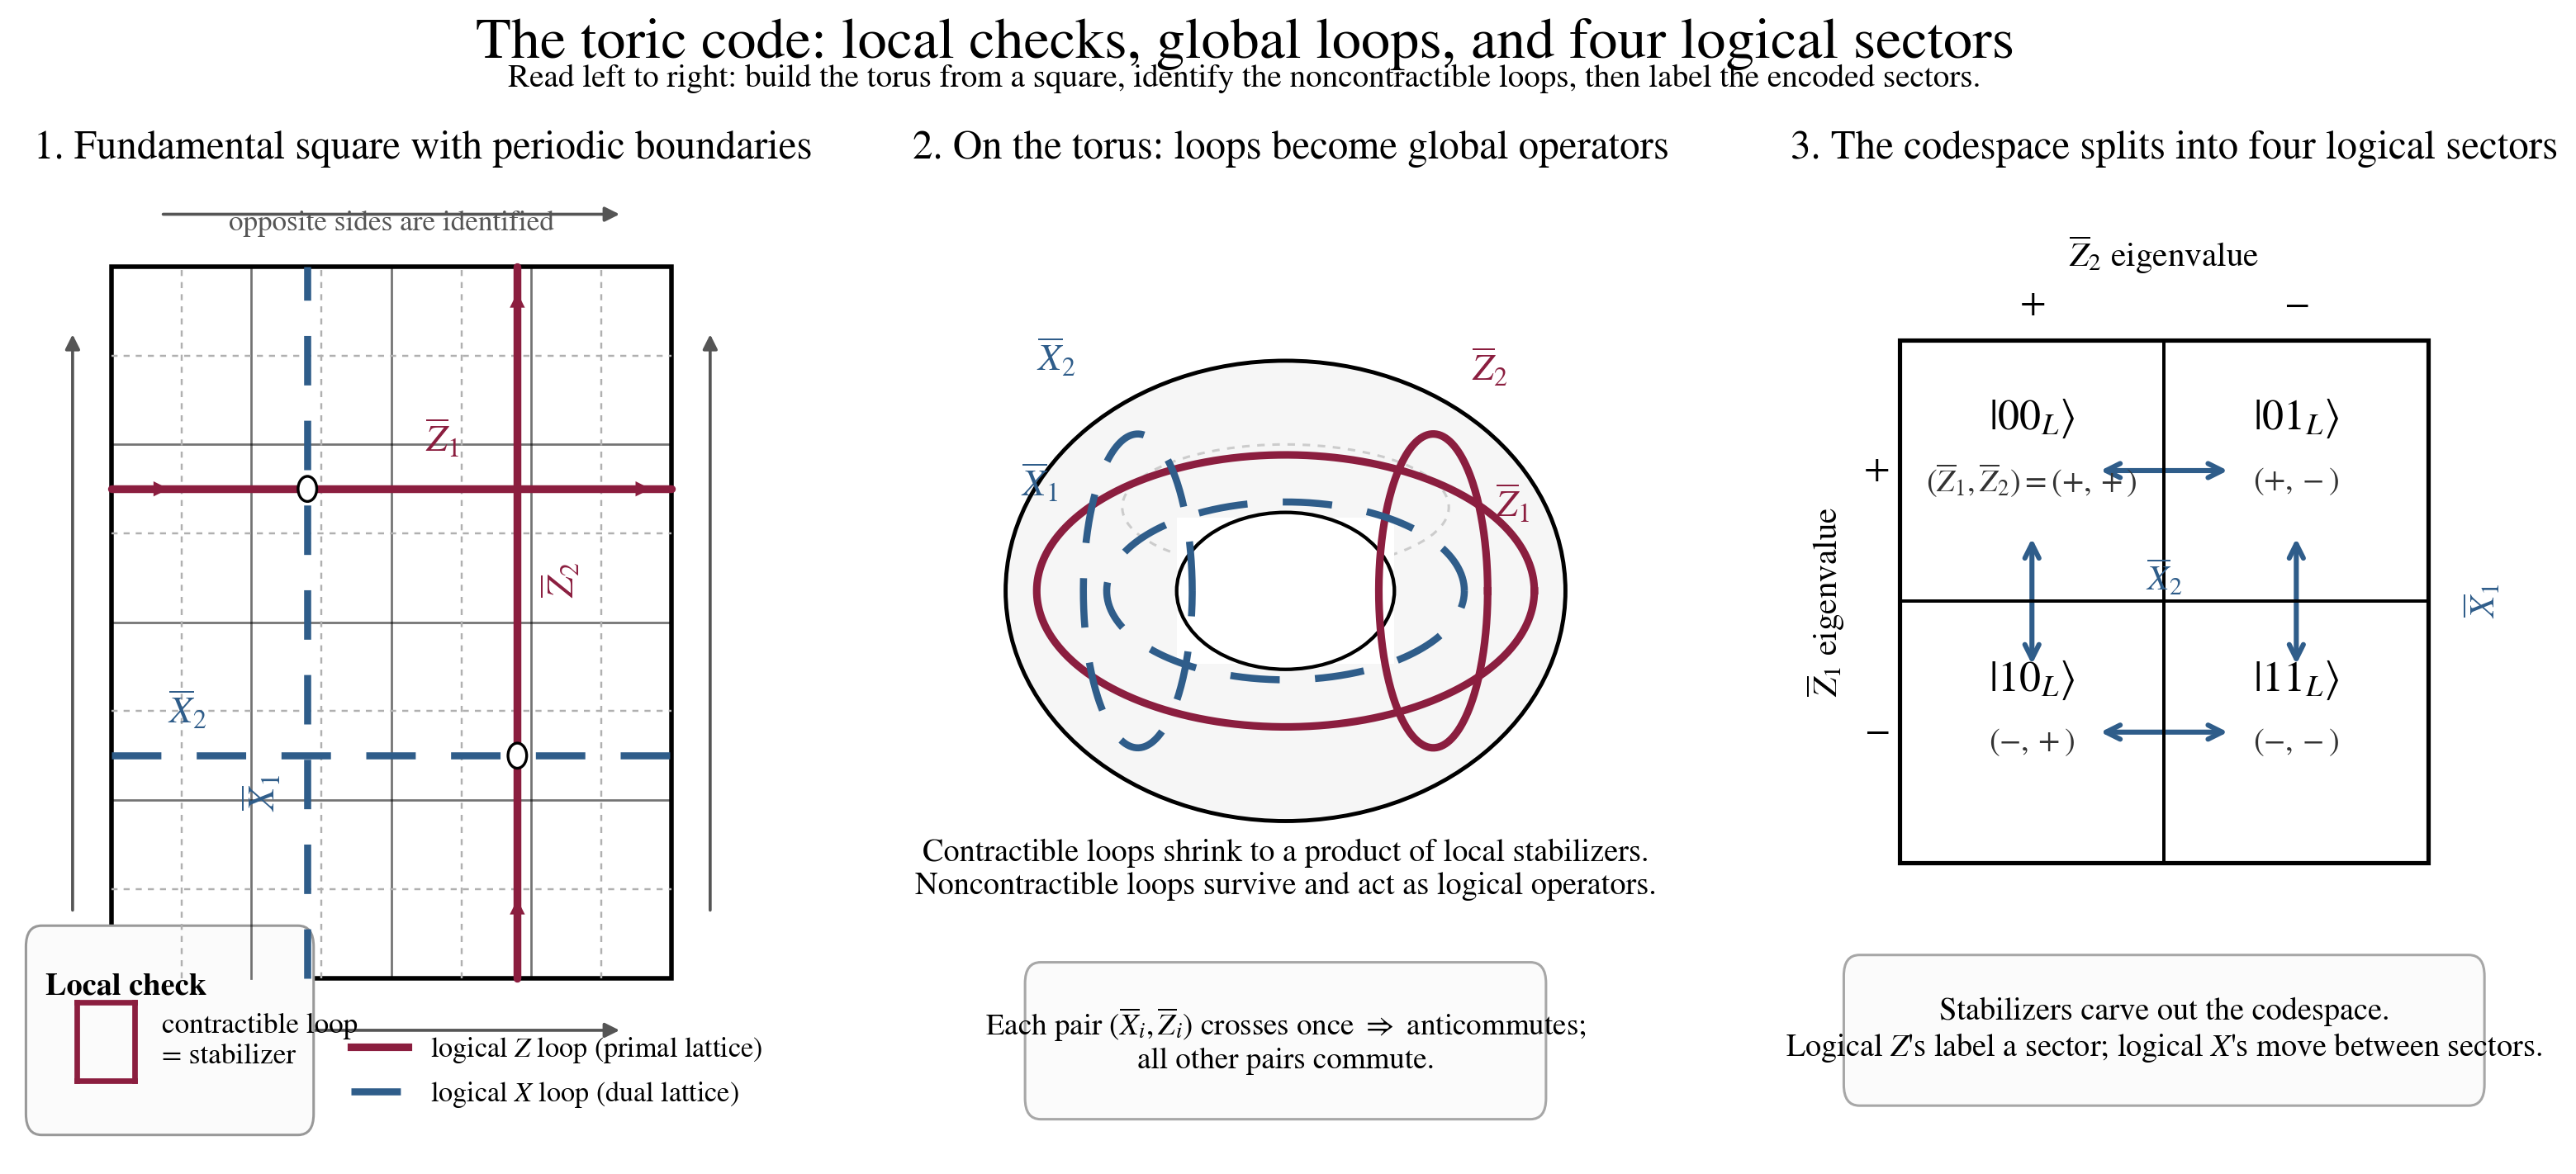
\includegraphics[width=0.84\linewidth]{toric_code_picture_first_diagram.png}
\caption{Picture-first toric-code dictionary.\label{fig:toric-picture-first}  Left: the fundamental square with opposite sides identified to form a torus. Middle: the two independent noncontractible directions, supporting logical $Z$-loops on the primal lattice and dual logical $X$-loops on the dual lattice. Right: the four logical sectors of the $k=2$ toric-code codespace, labeled by the eigenvalues of $(\overline Z_1,\overline Z_2)$.}
\end{figure}

\textbf{4. Higher cubical complexes and sheaf coefficients.}

Dinur--Lin--Vidick generalize the square-complex picture to arbitrary dimension $t$. The geometry is encoded as a \emph{graded incidence poset}, and the local algebra is encoded by a \emph{sheaf of coefficient spaces}.~\cite{DLV}

\begin{definition}[Higher cubical complex $X(G;\{A_i\})$]
Let $G$ be a finite set and let $A_1,\dots,A_t$ be finite sets of permutations of $G$, each closed under inverse, such that permutations taken from different $A_i$ pairwise commute. The associated cubical complex has vertex set
\[
G\times\{0,1\}^t,
\]
and, for each subset $S\subseteq [t]$ with $|S|=k$, a $k$-face of type $S$ is specified by data
\[
\bigl[g;(a_j)_{j\in S},(b_j)_{j\notin S}\bigr],
\qquad g\in G,\ a_j\in A_j,\ b_j\in\{0,1\},
\]
corresponding geometrically to the $2^k$ vertices
\[
\Bigl\{\bigl(g\cdot \prod_{j\in T}a_j,\;\beta(T,b)\bigr):T\subseteq S\Bigr\},
\]
where $\beta(T,b)\in\{0,1\}^t$ is the binary string whose $j$-th coordinate is $1$ if $j\in T$, $0$ if $j\in S\setminus T$, and $b_j$ if $j\notin S$. (The product $\prod_{j\in T}a_j$ is well-defined independent of ordering because elements of different $A_i$ commute by hypothesis.) The complex is naturally \emph{$2^t$-partite}; edges in direction $i$ come from $A_i$.~\cite{DLV}
\end{definition}

\begin{definition}[Graded incidence poset and local coefficients]
A graded poset $X$ with rank function $\rho$ is an \emph{incidence poset} if, whenever $f\preceq f''$ and $\rho(f'')=\rho(f)+2$, there are an even number of intermediate faces $f'$ with $f\prec\!\cdot\, f'\prec\!\cdot\, f''$. A system of local coefficients (or sheaf) on $X$ consists of:
\begin{itemize}
\item a finite-dimensional vector space $V_f$ for each face $f\in X$;
\item linear maps $F_{f\to f'}:V_f\to V_{f'}$ for each $f\succeq f'$ (restriction maps going from higher-rank faces to lower-rank sub-faces), satisfying
\[
F_{f'\to f''}\circ F_{f\to f'}=F_{f\to f''}
\qquad\text{whenever }f\succeq f'\succeq f''.
\]
\end{itemize}
\emph{Terminological note.} Because the maps go from larger cells to smaller sub-faces, this is technically a system of local coefficients on the opposite poset---what algebraic topologists would call a \emph{cosheaf}. The term ``sheaf'' is used throughout the coding-theory literature for this structure; a reader with a sheaf-theoretic background should read ``sheaf'' as ``cellular cosheaf'' or ``system of local coefficients'' throughout.
The associated chain groups are
\[
C_i(X,F):=\bigoplus_{f\in X(i)}V_f,
\]
and the boundary map is
\[
\partial_i(u)=\sum_{f'\prec\!\cdot\,f} \epsilon(f,f')\,F_{f\to f'}(u),\qquad u\in V_f\subseteq C_i(X,F),
\]
where $\epsilon(f,f')\in\{\pm 1\}$ is a sign assignment derived from a chosen orientation of faces (over $\mathbb F_2$ the signs are irrelevant and may be omitted; all applications in Sections~4 and~5 work over $\mathbb F_2$).
The compatibility and incidence conditions, together with the sign assignment, imply the fundamental chain-complex identity $\partial_{i-1}\partial_i=0$.~\cite{DLV}
\end{definition}

\begin{remark}[Why the graded incidence poset is needed]
This phrase is not just formalism. The \emph{graded} part is what lets us sort faces by dimension and define the chain groups
\[
C_i(X,F)=\bigoplus_{f\in X(i)}V_f.
\]
Without a grading, there is no coherent meaning to ``all $i$-faces,'' so the chain complex would not even be indexed correctly. The \emph{incidence} part is what makes ``boundary of boundary'' vanish: in every rank-$2$ interval $[f,f'']$, there are exactly two intermediate faces $f'_1,f'_2$, and the sign assignment is constructed so that
\[
\epsilon(f,f'_1)\epsilon(f'_1,f'')+\epsilon(f,f'_2)\epsilon(f'_2,f'')=0.
\]
This cancellation holds over \emph{any} field (it is a signed equality, not just a mod-2 cancellation), which is why the definition adds explicit signs $\epsilon(f,f')$. Over $\mathbb F_2$ the signs are redundant; for general $\mathbb F_q$ they are essential. Finally, the \emph{poset} language is the right level of generality because cubical faces are organized by inclusion, but the resulting geometry is not simplicial. In the higher cubical complexes $X(G;\{A_i\})$ of Dinur--Lin--Vidick, the face relation is proved to be a transitive graded partial order, and every rank-$2$ interval has exactly two intermediate faces; that is precisely why the construction yields an incidence poset and hence a genuine chain complex.~\cite{DLV}
\end{remark}

\begin{definition}[Cycle and cocycle expansion]
Let $C_*(X,F)$ be a chain complex with boundary $\partial$ and coboundary $\delta$. For $k\ge 0$, the \emph{cycle expansion} (equivalently, the local testability parameter for $k$-chains) is
\[
\varepsilon_{\mathrm{cyc}}(k):=\min_{x\in C_k(X,F)\setminus \ker \partial_k}
\frac{|\partial_k x|}{\operatorname{dist}(x,\ker \partial_k)},
\]
and the \emph{cocycle expansion} is
\[
\varepsilon_{\mathrm{cocyc}}(k):=\min_{x\in C^k(X,F)\setminus \ker \delta_k}
\frac{|\delta_k x|}{\operatorname{dist}(x,\ker \delta_k)}.
\]
Here $|\cdot|$ is the block-Hamming weight determined by the face support. A large $\varepsilon_{\mathrm{cyc}}(k)$ says that any chain far from being a $k$-cycle has a proportionally large boundary (soundness for $k$-chains); a large $\varepsilon_{\mathrm{cocyc}}(k)$ gives linear $k$-distance. These are the quantitative \emph{local-to-global parameters} used in the higher-cubical qLTC analysis.~\cite{DLV}
\end{definition}

\begin{definition}[Product expansion of a tuple of local codes]
Let $C_1,\dots,C_t\subseteq \mathbb F_q^n$ and write
\[
C^{(i)}:=\mathbb F_q^n\otimes\cdots\otimes C_i\otimes\cdots\otimes \mathbb F_q^n\subseteq \mathbb F_q^{[n]^t}
\]
for the subspace of tensors whose $i$-th slices all lie in $C_i$. Set
\[
C_1\boxplus\cdots\boxplus C_t \;:=\; \sum_{i=1}^t C^{(i)} \;\subseteq\; \mathbb F_q^{[n]^t},
\]
the (linear) sum of these $t$ subspaces. The tuple $(C_1,\dots,C_t)$ is \emph{$\rho$-product-expanding} if every $x\in C_1\boxplus\cdots\boxplus C_t$ admits a decomposition $x=\sum_{i=1}^t x_i$ with $x_i\in C^{(i)}$ satisfying
\[
\sum_{i=1}^t |x_i| \;\le\; \frac{1}{\rho}|x|,
\]
where $|\cdot|$ denotes Hamming weight in $\mathbb F_q^{[n]^t}$. Intuitively: every element of the sum can be efficiently expressed as a combination of axis-parallel components, with total component weight at most $(1/\rho)$ times the weight of the element. Large $\rho$ means efficient decompositions always exist. The precise formulation in~\cite{PKprod} is stated in terms of the number of nonzero axis-parallel lines; the Hamming-weight version above captures the same spirit. This is the higher-arity \emph{local algebraic hypothesis} feeding the cubical constructions.~\cite{PKprod}
\end{definition}

\textbf{5. Why the higher-dimensional step matters.}

The important point is that higher cubical complexes are \emph{not} just ``more boxes.'' They are a framework in which \emph{geometry and local algebra scale together}. The cubical complex supplies many compatible \emph{overlap patterns}; the sheaf supplies \emph{coefficient spaces and restriction maps}; the expansion parameters then control the resulting chain complex strongly enough to construct qLDPC codes (admitting single-shot decoders~\cite{GLZ}) and, at $t=4$, almost-good qLTCs.~\cite{DLV}

In that sense, the subject develops by repeatedly upgrading the same idea:
\[
\text{local consistency on a graph}
\Longrightarrow
\text{local tensor consistency on squares}
\Longrightarrow
\text{sheaf-valued consistency on }t\text{-cubes}.
\]
That is the conceptual content behind the modern phrase \emph{higher cubical complexes in quantum coding theory}. The cells become higher-dimensional, but more importantly the \emph{local-to-global mechanism} becomes richer, and that richer overlap is exactly what quantum coding theory exploits.

\begin{thebibliography}{9}\small
\bibitem{SS} M. Sipser and D. A. Spielman, \emph{Expander codes}, IEEE Transactions on Information Theory 42(6), 1710--1722, 1996.
\bibitem{Tanner1981} R. M. Tanner, \emph{A recursive approach to low complexity codes}, IEEE Transactions on Information Theory 27(5), 533--547, 1981.
\bibitem{Kitaev2003} A. Yu. Kitaev, \emph{Fault-tolerant quantum computation by anyons}, Annals of Physics 303(1), 2--30, 2003; preprint quant-ph/9707021, 1997.
\bibitem{DELLM} I. Dinur, S. Evra, R. Livne, A. Lubotzky, and S. Mozes, \emph{Locally testable codes with constant rate, distance, and locality}, STOC 2022 / arXiv:2111.04808.
\bibitem{QT} A. Leverrier and G. Z\'emor, \emph{Quantum Tanner codes}, FOCS 2022, arXiv:2202.13641.
\bibitem{GLZ} A. Gu, A. Leverrier, and G. Z\'emor, \emph{Single-shot decoding of good quantum LDPC codes}, arXiv:2306.12470, 2023.
\bibitem{DLV} I. Dinur, T.-C. Lin, and T. Vidick, \emph{Expansion of high-dimensional cubical complexes with application to quantum locally testable codes}, arXiv:2402.07476.
\bibitem{PKprod} G. Kalachev and P. Panteleev, \emph{Maximally extendable product codes are good coboundary expanders}, FOCS 2025 version / arXiv:2501.01411.
\bibitem{Gottesman1997} D. Gottesman, \emph{Stabilizer codes and quantum error correction}, Ph.D.\ thesis, California Institute of Technology, 1997; arXiv:quant-ph/9705052.
\bibitem{CS1996} A. R. Calderbank and P. W. Shor, \emph{Good quantum error-correcting codes exist}, Physical Review A 54(2), 1098--1105, 1996; A. M. Steane, \emph{Error correcting codes in quantum theory}, Physical Review Letters 77(5), 793--797, 1996.
\bibitem{WLH} A. Wills, T.-C. Lin, and M.-H. Hsieh, \emph{Tradeoff constructions for quantum locally testable codes}, IEEE Trans. Inform. Theory 71 (2025).
\end{thebibliography}

\end{document}